\documentclass[aspectratio=169]{beamer}
\setbeamertemplate{navigation symbols}{}
\usepackage{color, amsmath, comment, subfigure}
\usepackage{url}

\usepackage{hyperref}
\hypersetup{
    colorlinks=true,
    linkcolor=blue,
    filecolor=magenta,      
    urlcolor=cyan,
}

%%%%%%%%%%%%%%%%%%%%%%%%%%
\title[]{Preread slides for Thursday, Sept 24:\\Armed conflict, part 2}
\author[]{Matthew J. Salganik}
\institute[]{}
\date[]{COS 597E/SOC 555 Limits to prediction\\Fall 2020, Princeton University}

\begin{document}
%%%%%%%%%%%%%%%%%%%%%%%%%%%
\frame{\titlepage}
%%%%%%%%%%%%%%%%%%%%%%%%%%%
\begin{frame}
\frametitle{}

\begin{center}
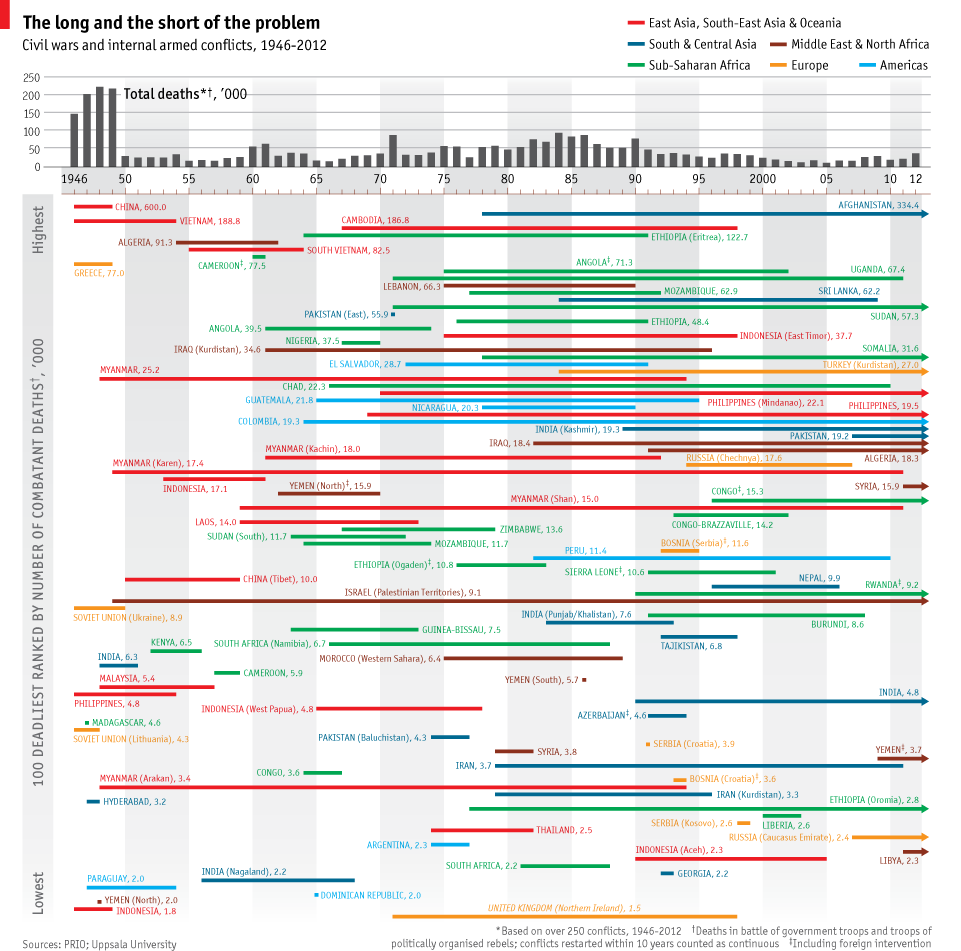
\includegraphics[height=0.9\textheight]{figures/ourworldindata_the-100-deadlist-civil-wars-the-economist}
\end{center}

\vfill
\tiny{\url{https://www.economist.com/content/inner-turmoil}}
% focus on onset
\end{frame}
%%%%%%%%%%%%%%%%%%%%%%%%%%%%
\begin{frame}
\frametitle{}

\begin{center}
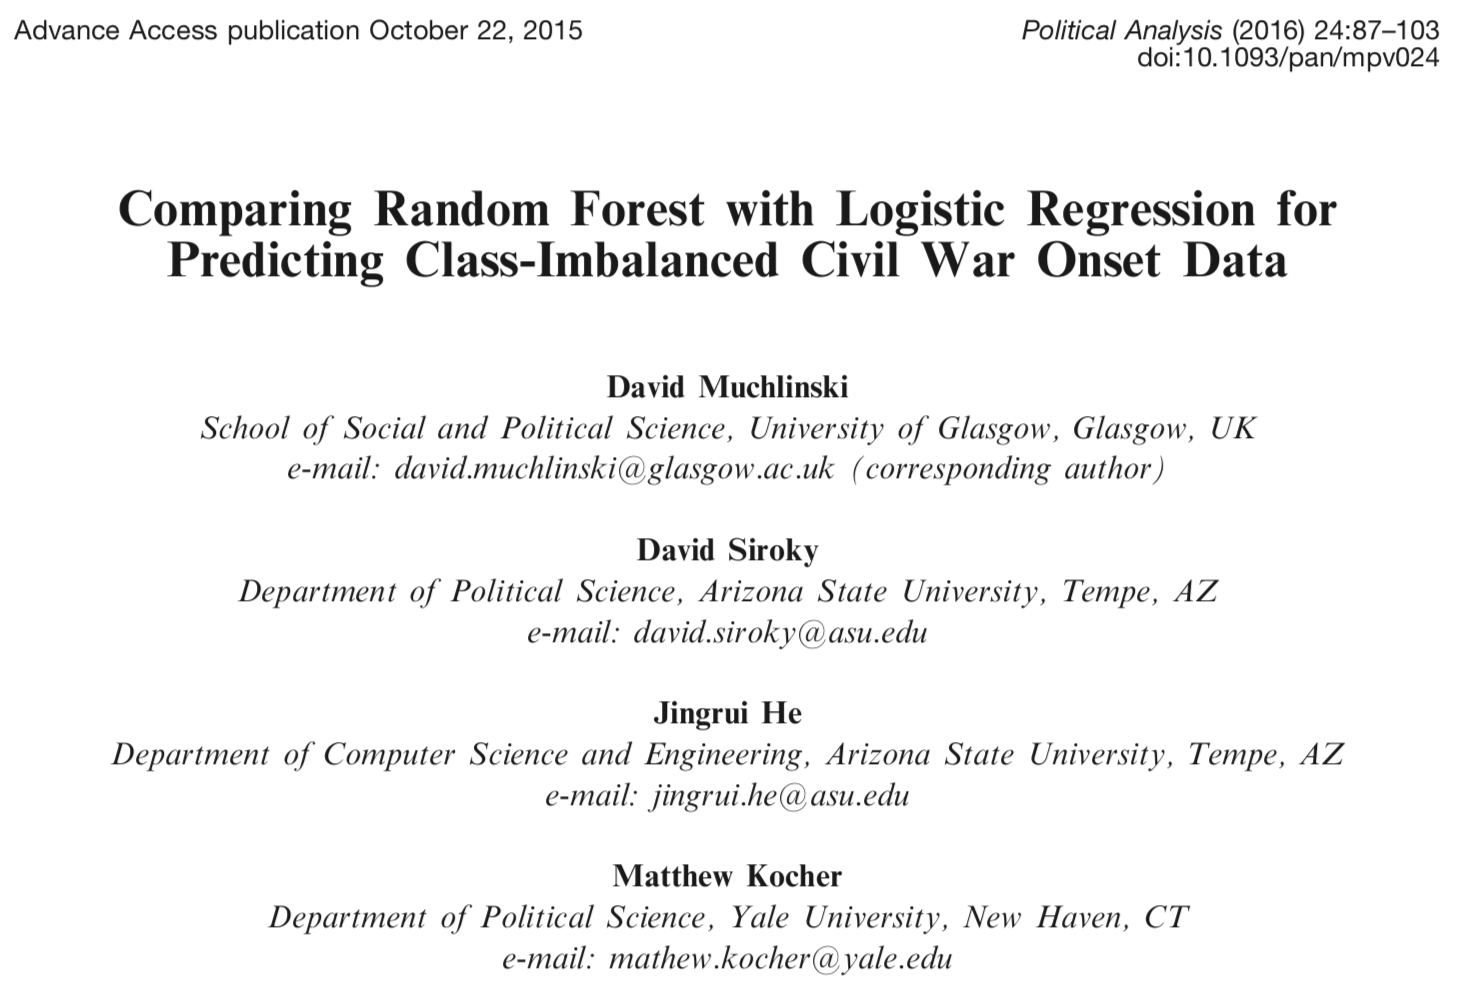
\includegraphics[width=0.9\textwidth]{figures/muchlinksi_comparing_2016_title}
\end{center}

\end{frame}
%%%%%%%%%%%%%%%%%%%%%%%%%%%%
\begin{frame}

Reading notes:
\begin{itemize}
\item Major goals: (1) compare random forest to logistic regression for predicting civil war onset (2) learn from random forest about civil war onset.
\pause
\item For goal (1), note that two things are varying: number of predictors and learning algorithm. 
\pause
\item For goal (1), think about the role of time in assessing predictions.
\pause
\item For goal (2), ask yourself if you believe the results in Fig 4 and 5. It is OK if you don't have strong feelings either way. 
\pause
\item Note that this starts off like a paper about civil wars and seems to end up like a paper about random forest.
\pause
\item Do you see any connection to idea of theoretical limits?
\end{itemize}

\end{frame}
%%%%%%%%%%%%%%%%%%%%%%%%%%%
\begin{frame}

Many responses.  Reading notes:
\begin{itemize}
\item Neenhoeffer and Sternberg: How to measure generalization? Are we cheating with our cross-validation? How many training loops are there? Questions about cross-validation go beyond the ones raised here.  This might feel like the weeds, but it is hard to quantitatively study the limits of predictability if we cannot clearly and accurately measure predictability.
\pause
\item Don't worry so much about the other responses.
\pause
\item Note the value of open and reproducible research.
\pause
\item Do you find the authors' reply convincing?
\end{itemize}

\end{frame}
%%%%%%%%%%%%%%%%%%%%%%%%%%%
\frame{\titlepage}


\end{document}
